\documentclass{article}
\usepackage{graphicx} % Required for inserting images
\usepackage{amsmath}
\usepackage{amssymb} % used for math symbols
\usepackage{mathtools}
\usepackage{svg}

\makeatletter
\newcommand*{\rom}[1]{\expandafter\@slowromancap\romannumeral #1@}
\makeatother

\title{Computer Grafik Blatt 5}
\date{May 2023}

% disable paragraph indentation
\setlength{\parindent}{0pt}

\begin{document}

\maketitle

\section*{Aufgabe 1}

\subsection*{a)}
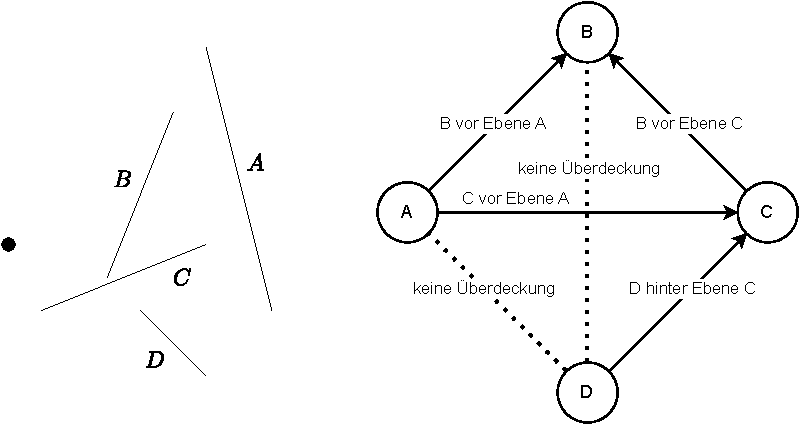
\includegraphics[width=\textwidth, keepaspectratio]{aufgabe01a.2.drawio.pdf}
\\
Daraus ergeben sich die Reihenfolgen $A,D,C,B$ bzw. $D,A,C,B$

\subsection*{b)}
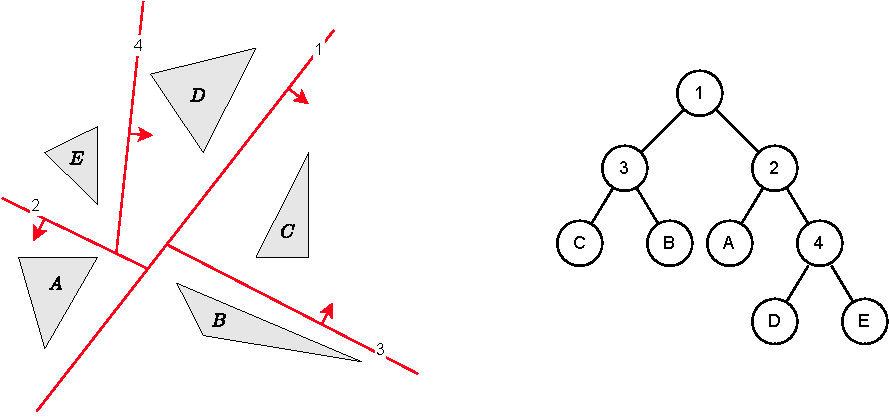
\includegraphics[width=\textwidth, keepaspectratio]{aufgabe01b.2.drawio.pdf}

\subsection*{c)}
$x = \begin{pmatrix}4 \\ 1 \\ 3 \end{pmatrix}$, $\vec{w} = \begin{pmatrix} -\frac{1}{\sqrt{2}} \\ 0 \\ -\frac{1}{\sqrt{2}} \end{pmatrix}$ \\
$a = \begin{pmatrix} 0 \\ 0 \\ 0 \end{pmatrix}$, $b = \begin{pmatrix} 3 \\ 0 \\ 0 \end{pmatrix}$, $c = \begin{pmatrix} 0 \\ 2 \\ -1 \end{pmatrix}$ \\
Normale des Dreiecks bestimmen:
\begin{align*}
    n & = \frac{(b-a) \times (c-a)}{||(b-a) \times (c-a)||}                                                                                                 \\
      & = \begin{pmatrix} 3 - 0 \\ 0 - 0 \\ 0 - 0 \end{pmatrix} \times \begin{pmatrix} 0 - 0 \\ 2 - 0 \\ -1 - 0 \end{pmatrix} \div ||(b-a) \times (c-a)|| \\
      & = \begin{pmatrix} 3 \\ 0 \\ 0 \end{pmatrix} \times \begin{pmatrix} 0 \\ 2 \\ -1 \end{pmatrix} \div ||(b-a) \times (c-a)||                     \\
      & = \begin{pmatrix} 0 \\ 3 \\ 6 \end{pmatrix} \div \sqrt{0^2 + 3^2 + 6^2} \\
      & = \begin{pmatrix} 0 \\  \frac{\sqrt{5}}{5} \\ \frac{2\sqrt{5}}{5} \end{pmatrix}
\end{align*}

% TODO: Forgot to normalize the normal vector >:(
Mit Normale Schnittpunkt von Gerade und Dreiecksebene bestimmen:
\begin{align*}
    n^T \cdot (x + \lambda \vec{w} - a) & = 0                                                                                                                                                                                                                                                        \\
    \lambda                             & = \frac{n^T \cdot (a - x)}{n^T \cdot \vec{w}}                                                                                                                                                                                                              \\
                                        & = \frac{\begin{pmatrix} 0 & \frac{\sqrt{5}}{5} &  \frac {2\sqrt{5}}{5} \end{pmatrix} \cdot \begin{pmatrix} -4 \\ -1 \\ -3 \end{pmatrix}}{\begin{pmatrix} 0 & \frac{\sqrt{5}}{5} &  \frac {2\sqrt{5}}{5} \end{pmatrix} \cdot \begin{pmatrix} -\frac{1}{\sqrt{2}} \\ 0 \\ -\frac{1}{\sqrt{2}} \end{pmatrix}} \\
                                        & = \frac{-\frac{7\sqrt{5}}{5}}{-\frac{\sqrt{10}}{5}}                                                                                                                                                                                                                                    \\
                                        & = -\frac{7\sqrt{2}}{2} \approx 4.95
\end{align*}

Damit ergibt sich der Punkt $p = \begin{pmatrix} 4 \\ 1 \\ 3 \end{pmatrix} + \frac{7\sqrt{2}}{2} \cdot \begin{pmatrix} -\frac{1}{\sqrt{2}} \\ 0 \\ -\frac{1}{\sqrt{2}} \end{pmatrix} = \begin{pmatrix} \frac{1}{2} \\ 1 \\ -\frac{1}{2} \end{pmatrix}$

Mit Hilfe der baryzentrischen Koordinaten prüfen, ob der Punkt im Dreieck liegt:

\[
    \begin{aligned}
        A(\triangle_{abc}) & = \frac{1}{2} \cdot det \begin{pmatrix}
                                                         |   & |   & |             \\
                                                         b-a & c-a & n_{\triangle} \\
                                                         |   & |   & |
                                                     \end{pmatrix} \\
                           & = \frac{1}{2} \cdot det \begin{pmatrix}
                                                         3 & 0  & 0 \\
                                                         0 & 2  & 3 \\
                                                         0 & -1 & 6
                                                     \end{pmatrix}            \\
                           & = \frac{1}{2} \cdot 45 = 22.5                     \\
                           &                                                   \\
                           &                                                   \\
        A(\triangle_{pbc}) & = \frac{1}{2} \cdot det \begin{pmatrix}
                                                         |   & |   & |             \\
                                                         b-p & c-p & n_{\triangle} \\
                                                         |   & |   & |
                                                     \end{pmatrix} \\
                           & = \frac{1}{2} \cdot det \begin{pmatrix}
                                                         2.5 & -0.5 & 0 \\
                                                         -1   & 1    & 3 \\
                                                         0.5 & -0.5 & 6
                                                     \end{pmatrix}           \\
                           & = \frac{1}{2} \cdot 15 = 7.5                   \\
                           &                                                   \\
                           &                                                   \\
        A(\triangle_{pca}) & = \frac{1}{2} \cdot det \begin{pmatrix}
                                                         |   & |   & |             \\
                                                         c-p & a-p & n_{\triangle} \\
                                                         |   & |   & |
                                                     \end{pmatrix} \\
                           & = \frac{1}{2} \cdot det \begin{pmatrix}
                                                         -0.5 & -0.5 & 0 \\
                                                         1    & -1   & 3 \\
                                                         -0.5 & 0.5 & 6
                                                     \end{pmatrix}           \\
                           & = \frac{1}{2} \cdot 7.5 = 3.75                  \\
                           &                                                   \\
                           &                                                   \\
        A(\triangle_{pab}) & = \frac{1}{2} \cdot det \begin{pmatrix}
                                                         |   & |   & |             \\
                                                         a-p & b-p & n_{\triangle} \\
                                                         |   & |   & |
                                                     \end{pmatrix} \\
                           & = \frac{1}{2} \cdot det \begin{pmatrix}
                                                         -0.5 & 2.5 & 0 \\
                                                         -1   & -1   & 3 \\
                                                         0.5 & 0.5 & 6
                                                     \end{pmatrix}           \\
                           & = \frac{1}{2} \cdot 22.5 = 11.25                \\
    \end{aligned}
\]

\[
    \begin{aligned}
        \alpha &= \frac{A(\triangle_{pbc})}{A(\triangle_{abc})} = \frac{7.5}{22.5} = \frac{1}{3}\\
        \beta  &= \frac{A(\triangle_{pca})}{A(\triangle_{abc})} = \frac{3.75}{22.5} = \frac{1}{6}\\
        \gamma &= \frac{A(\triangle_{pab})}{A(\triangle_{abc})} = \frac{11.25}{22.5} = \frac{1}{2}
    \end{aligned}
\]

Positive baryzentrische Koordinaten für $p$ Zeigen, dass $p$ im Dreieck liegt. 
Somit ist der Schnittpunkt $p=\begin{pmatrix} \frac{1}{2} \\ 1 \\ -\frac{1}{2} \end{pmatrix}$

\subsection*{d)}
z-Buffer initial mit $1$ und color-Buffer mit $(1,1,1)$ füllen. \\
\begin{enumerate}
    \item $[z = 0.2; c = (0.7, 0.7, 0)]$
          \begin{itemize}
              \item $\text{z-Buffer} = 0.2;\ \text{color-Buffer} = (0.7, 0.7, 0)$
          \end{itemize}
    \item $[z = 0.4; c = (0, 0, 0)]$
          \begin{itemize}
              \item $\text{z-Buffer} = 0.2;\ \text{color-Buffer} = (0.7, 0.7, 0)$
          \end{itemize}
    \item $[z = 0.9; c = (0.1, 0.2, 0.9)]$
          \begin{itemize}
              \item $\text{z-Buffer} = 0.2;\ \text{color-Buffer} = (0.7, 0.7, 0)$
          \end{itemize}
    \item $[z = -0.3; c = (0.1, 0.9, 1)]$
          \begin{itemize}
              \item $\text{z-Buffer} = -0.3;\ \text{color-Buffer} = (0.1, 0.9, 1)$
          \end{itemize}
    \item $[z = -0.8; c = (0, 1, 0.8)]$
          \begin{itemize}
              \item $\text{z-Buffer} = -0.8;\ \text{color-Buffer} = (0, 1, 0.8)$
          \end{itemize}
\end{enumerate}

\subsection*{e)}
$\alpha$-Buffer initial mit $0$ füllen und color-Buffer mit $(1,1,1)$ füllen. \\

\begin{enumerate}
    \item $[z = 0.2; c = (0.1, 0.1, 0.1), \alpha = 0.2]$
    \item $[z = -1.0; c = (0, 1, 1), \alpha = 0.8]$
    \item $[z = -0.3; c = (0, 1, 0), \alpha = 1.0]$
    \item $[z = 0.6; c = (0.7, 0.8, 0.9), \alpha = 0.2]$
    \item $[z = 0.2; c = (1, 1, 1), \alpha = 0.5]$
\end{enumerate}

Fragmente vom großen zum kleinen z-Wert sortieren, da große Werte hinten und kleine Werte vorne liegen.
Entsprechend der Formel $C_i = \alpha_i \cdot c_i + (1 - \alpha_i) \cdot C_{i-1}$ berechnet, beginnend mit $C_0 = (1,1,1)$: \\
\begin{enumerate}
     \item $[z = 0.6;\ c = (0.7, 0.8, 0.9);\ \alpha = 0.2]$
    \begin{itemize}
        \item $C_1 = 0.2 \cdot (0.7, 0.8, 0.9) + (1 - 0.2) \cdot (1, 1, 1) = (0.94, 0.96, 0.98)$
    \end{itemize}
    \item $[z = 0.2;\ c = (0.1, 0.1, 0.1);\ \alpha = 0.2]$
    \begin{itemize}
        \item $C_2 = 0.2 \cdot (0.1, 0.1, 0.1) + (1 - 0.2) \cdot (0.94, 0.96, 0.98) = (0.772, 0.788, 0.804)$
    \end{itemize}
    \item $[z = -0.2;\ c = (1, 1, 1);\ \alpha = 0.5]$
    \begin{itemize}
        \item $C_3 = 0.5 \cdot (1, 1, 1) + (1 - 0.5) \cdot (0.772, 0.788, 0.804) = (0.886, 0.894, 0.902)$
    \end{itemize}
    \item $[z = -0.3;\ c = (0, 1, 0);\ \alpha = 1.0]$
    \begin{itemize}
        \item $C_4 = 1.0 \cdot (0, 1, 0) + (1 - 1.0) \cdot (0.886, 0.894, 0.902) = (0.0, 1.0, 0.0)$
    \end{itemize}
    \item $[z = -1.0;\ c = (0, 1, 1);\ \alpha = 0.8]$
    \begin{itemize}
        \item $C_5 = 0.8 \cdot (0, 1, 1) + (1 - 0.8) \cdot (0.0, 1.0, 0.0) = (0.0, 1.0, 0.8)$
    \end{itemize}
\end{enumerate}
   
Somit erhalten wir $ (0.0, 1.0, 0.8)$ als Ergebnis.

\end{document}